\documentclass{standalone}
% main document, called main.tex

% \usepackage{newtxtext}       %
% \usepackage{newtxmath}   
\usepackage{amsmath}   
\usepackage{amssymb}   

\newcommand\szcirc{0.36cm}

\usepackage{tikz}

\begin{document}

\newcommand{\juv}{S}

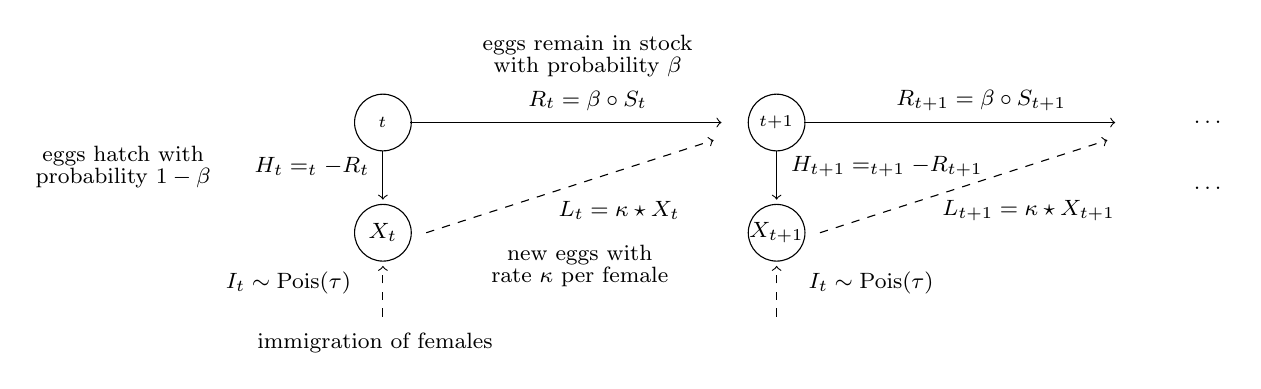
\begin{tikzpicture}[x=1cm,y=0.28cm]
\footnotesize
% two place holders to get some margins:
% \draw[white,fill=white](6,1) node {};
% \draw[white,fill=white](6,1) node {};

% circles:
\draw[black,fill=white](11,1) circle (\szcirc) node {$\juv_{t}$};
% \draw[black,fill=white](11,-3) circle (\szcirc) node {$H_{t}$};

\draw[black,fill=white](11,-4) circle (\szcirc) node {$X_{t}$};
% \draw[black,fill=white](11,-11) circle (\szcirc) node {$I_{t}$};

\draw[black,fill=white](16,1) circle (\szcirc) node {$\juv_{t + 1}$};
% \draw[black,fill=white](16,-3) circle (\szcirc) node {$H_{t + 1}$};
\draw[black,fill=white](16,-4) circle (\szcirc) node {$X_{t + 1}$};
% \draw[black,fill=white](16,-11) circle (\szcirc) node {$I_{t + 1}$};

% dots right
\draw[black,fill=white](21.5,1) node {$\dots$};
\draw[black,fill=white](21.5,-2) node {$\dots$};

% long horizontal arrows:
\foreach \x/\y in {11/15.3, 16/20.3}
{\draw[->] (\x.35,1) -- (\y,1);}


% vertical arrows:
\foreach \x in {11, 16}
{\draw[->] (\x, -0.3) -- (\x, -2.5);
\draw[->, dashed] (\x, -7.8) -- (\x, -5.5);
% \draw[->, double distance=0.5pt] (\x, -9.7) -- (\x, -8.5);
}

% diagonal arrows:
\foreach \x in {11, 16}
{\draw[->, dashed] (\x + 0.55, -4) -- (\x + 4.2, 0.2);
}

% text
\draw[black,fill=white](7.7,-0.5) node {eggs hatch with};
\draw[black,fill=white](7.7,-1.5) node {probability $1 - \beta$};
\draw[black,fill=white](10.1,-1) node {$H_t = \juv_t - R_t$};
\draw[black,fill=white](9.8,-6.3) node {$I_t \sim \text{Pois}(\tau)$};

\draw[black,fill=white](17.4,-1) node {$H_{t + 1} = \juv_{t + 1} - R_{t + 1}$};
\draw[black,fill=white](17.2,-6.3) node {$I_t \sim \text{Pois}(\tau)$};



\draw[black,fill=white](10.9,-9) node {immigration of females};
% \draw[black,fill=white](10.5,-9.5) node {to Pois($\tau$)};

\draw[black,fill=white](13.6,4.5) node {eggs remain in stock};
\draw[black,fill=white](13.6,3.5) node {with probability $\beta$};
\draw[black,fill=white](13.6,2) node {$R_t = \beta \circ S_t$};
\draw[black,fill=white](18.6,2) node {$R_{t + 1} = \beta \circ S_{t + 1}$};


\draw[black,fill=white](14,-3) node {$L_t = \kappa \star X_t$};
\draw[black,fill=white](13.5,-5) node {new eggs with};
\draw[black,fill=white](13.5,-6) node {rate $\kappa$ per female};
\draw[black,fill=white](19.2,-3) node {$L_{t + 1} = \kappa \star X_{t + 1}$};

\end{tikzpicture}

\end{document}